% vim: tw=78 encoding=utf8 ts=2 sw=2 expandtab softtabstop=2
\documentclass[11pt,twocolumn,a4paper,english]{article}

\usepackage[utf8]{inputenc}
\usepackage{babel}
\usepackage{url}
\usepackage{graphicx}
\usepackage{anysize}
\marginsize{1.7cm}{1.7cm}{1.7cm}{1.7cm}

\newcommand{\TODO}{\textbf{TODO:} }

\title{
Synthesizing Benchmarks for Architecture Recovery Algorithms}
\author{Rodrigo Souza \\ rodrigorgs@gmail.com 
\and Dalton Guerrero \\ dalton@dsc.ufcg.edu.br
\and Jorge Figueiredo \\ abrantes@dsc.ufcg.edu.br
\and Christina Chavez \\ flach@ufba.br
}

\begin{document}

\sloppy
\maketitle

\TODO Redo some figures to fit better in a two column paper.

\TODO Display authors in a 2x2 matrix.

% TODO entrada do BCR+ é uma arquitetura de referência.

\begin{abstract}
	As a software system evolves, its actual architecture may deviate from its original reference architecture. A better understanding of the actual architecture can be gained by applying architecture recovery algorithms to the source code of the system. Unfortunately, there is little knowledge regarding the quality of such algorithms, mostly because, in order to assess their accuracy, one needs updated, detailed architectures for a variety of software systems.
	To overcome such problem, we propose a simulation model that synthesizes implementation-level dependency graphs that conform to the module view of any given reference architecture. We show, using observations from network theory, that the graphs are very similar to dependency graphs extracted from the source code of real software systems. 
	Then, we synthesize thousands of graphs, in a controlled way, and use them as benchmarks for six well-known architecture recovery algorithms: ACDC, Bunch, SL75, SL90, CL75, and CL90. By comparing the given reference architectures with those recovered by the algorithms, we conclude that ACDC and Bunch outperform the alternatives, specially if the architecture contains more than a couple of modules.\end{abstract}

%%%%%%%%%%%%%%%%%%%%%%%%%%%%%%%%%%%%%%%%%%%%%%%%%%%%%%%%%%%%%%%%%%%%%%%%%%%%%
%%%%%%%%%%%%%%%%%%%%%%%%%%%%%%%%%%%%%%%%%%%%%%%%%%%%%%%%%%%%%%%%%%%%%%%%%%%%%

% I use begin/end instead of just \section so I can fold sections in my text editor
\begin{section}{Introduction}
% This section should be succinct, with no subheadings
	Architectural drift

	Reverse engineering / Architecture recovery algorithms
	
	Architecture recovery / discovery / reconstruction
	
	Architecture recovery algorithms have been used as a starting point to recover the reference architecture of a system family (Recovery of a Reference Architecture: A case study, by Eixelsberger / Architecture Recovery for Product Families, by Pinzger et al / Enhancing Domain-Specific Software Architecture Recovery, by Ivkovic and Godfrey) 
	([LIMBO] Improving the build architecture of legacy C/C++ software systems, by Dayani-Fard et al / [Bunch] ).
	
	One such kind of algorithms are the software clustering algorithms. They help to recover the module viewpoint of an architecture. They tend to find high cohesive clusters with low coupling between clusters. However, little is known about the performance of such algorithms on software. 
	
\end{section}

%%%%%%%%%%%%%%%%%%%%%%%%%%%%%%%%%%%%%%%%%%%%%%%%%%%%%%%%%%%%%%%%%%%%%%%%%%%%%

\begin{section}{Background}
	Architecture recovery algorithms

	Evaluation of architecture recovery algorithms. 
	
\end{section}

%%%%%%%%%%%%%%%%%%%%%%%%%%%%%%%%%%%%%%%%%%%%%%%%%%%%%%%%%%%%%%%%%%%%%%%%%%%%%

\begin{section}{Proposed solution}
	
	Goal: analyze or compare architecture recovery algorithms in different contexts.
	
	Research approach:
	
	\begin{itemize}
		\item Create a model that synthesizes graphs that are similar to software dependency graphs, given a reference architecture
		
		\begin{itemize}
			\item Create a graph classifier, that determines if a graph is likely to be a software dependency graph (i.e., if it is software-realistic)
			\item Evaluate the classifier, in terms of precision and recall
			\item Using the classifier, determine if the model synthesizes software-realistic graphs 
		\end{itemize}		
	\end{itemize}
	
	Usage (exemplified in our proof of concept):
	
	\begin{itemize}
		\item Use the model to synthesize a variety of graphs. 

		\item Apply architecture recovery algorithms to the graphs.

		\item Compare recovered with reference architectures.

		\item Analyze.
	\end{itemize}
	
	
\end{section}

%%%%%%%%%%%%%%%%%%%%%%%%%%%%%%%%%%%%%%%%%%%%%%%%%%%%%%%%%%%%%%%%%%%%%%%%%%%%%

\begin{section}{The BCR+ model}	
	\newcommand{\din}[0]{\ensuremath{\delta_{in}}}
	\newcommand{\dout}[0]{\ensuremath{\delta_{out}}}
	\newcommand{\gin}[0]{\ensuremath{\mathrm{g}_{in}}}
	\newcommand{\gout}[0]{\ensuremath{\mathrm{g}_{out}}}
	
	\TODO Talk about network theory / complex networks / scale-free networks 
  %TODO Chris:	mv to background

	When designing the architecture of a software system, the module viewpoint plays a major role, by specifying the modules of the system and their inter-relationships. Constraining such dependencies benefits the maintenatibility, portability, and reusability of the software system.
	
	In this section, we describe the BCR+ model for synthesizing graphs from a description of the module viewpoint of an arbitrary architecture --- that is, the modules and dependencies between modules. The BCR+ model produces---by means of the mechanisms of growth and preferential attachment---directed graphs that are both scale-free and segmented in modules.
	
	\TODO there are other models, but they don't take architecture as input	
	
\begin{subsection}{Overview}
	The BCR+ model is a generalization of a graph model proposed by Bollobás et al \cite{Bollobas2003}. The original model generates directed graphs that are scale-free. Our model extends the original by generating graphs in which the nodes are organized in modules, according to an modular architecture given as input.
	
	The BCR+ model takes the following parameters as input:
	
	\begin{itemize}
  \item number of vertices, $n$;
  \item three probability values, $p_1$, $p_2$ e $p_3$, com $p_1 + p_2 + p_3 = 1$;
  \item base in-degree, $\din$;
  \item base out-degree, $\dout$.
  \item an directed graph representing dependencies between modules, $G$;
  \item a constant, $\mu$, with $0,0 \le \mu \le 1,0$;
  \end{itemize}
  
	The last two parameters are new in BCR+. The other ones are from the original model by Bollobás et al \cite{Bollobas2003}.
	
	In the graph $G$, each vertex represents one module of the architecture. Each edge defines a relationship of dependency between modules. We say that a module $M_1$ depends on another module, $M_2$, if $G$ contains an edge from the vertex that represents $M_1$ to the vertex that represents $M_2$. In the graph that is created, an edge from a vertex $v_1 \in M_1$ to another vertex, $v_2 \in M_2$, can be created only if $M_1$ depends on $M_2$ in the graph $G$ or if $M_1$ and $M_2$ are the same module.
	
		\TODO Say that these graphs contain both internal and external edges. Define internal/external.
		
	The parameter $\mu$ controls the proportion of external edges in the graph---that is, edges connecting vertices in distinct modules. Lower values lead to graphs with fewer external edges.
	
	The original model by Bollobás et al \cite{Bollobas2003} is a particular case of BCR+ when $\mu = 0$ and $G$ contains one single vertex, representing one single module.
	

\begin{figure*}[htbp]
	\centering
		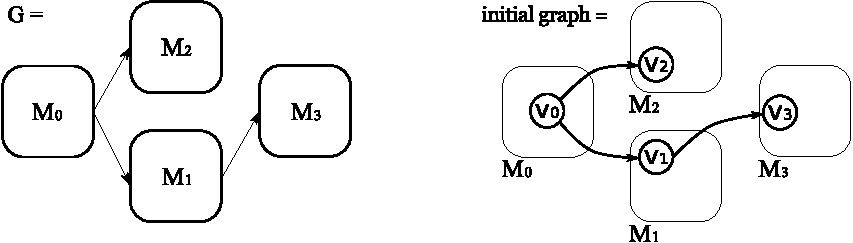
\includegraphics[scale=1]{figures/bcr-initial-graph}
	\caption{Initial graph synthesized by BCR+, given an input graph parameter $G$.}
	\label{fig:bcr-initial-graph}
\end{figure*}
	
	As a computer model, BCR+ takes the parameters as inputs and, by running an algorithm, outputs a graph. The algorithm builds the output graph incrementally. It starts by creating a module for each vertex in the input graph $G$, and then adding one vertex to each module. After that, it creates all external edges that are allowed by $G$ (see Figure \ref{fig:bcr-initial-graph}). Then, the graph is modified according to three formation rules that are applied successively, in random order, until the graph grows to $n$ vertices. At each algorithm step, the probability of the $i$-th being applied is given by the parameter $p_i$.

\end{subsection}	

\begin{subsection}{Formation Rules}
	
	There are three formation rules in BCR+. Each one modifies the output graph by adding or removing vertices or edges in the graph. Also, each formation rule has a probability of being applied, given by the parameters $p_1$, $p_2$ and $p_3$.

\begin{figure*}[htbp]
	\centering
		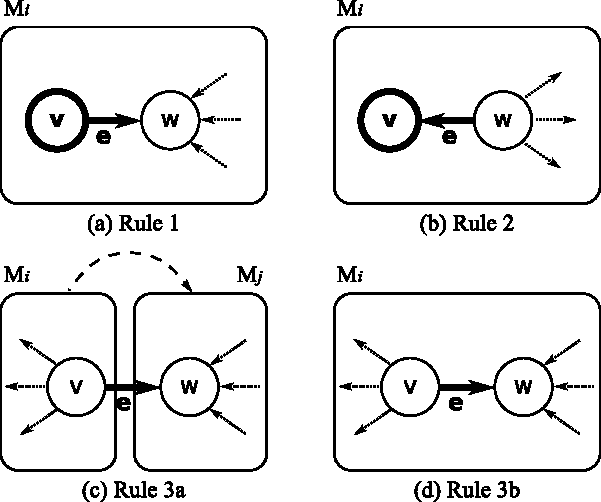
\includegraphics[scale=1]{figures/bcr-rules}
	\caption{Formation rules for BCR+. $M_i$ and $M_j$ are distinct modules, such as $M_i$ depends on $M_j$. In the diagram for each rule, thicker lines represent vertices and edges created when the rule is applied.}
	\label{fig:bcr-rules}
\end{figure*}

	The rules are illustrated in Figure \ref{fig:bcr-rules}. Simplified rules:
	
	\begin{itemize}
		\item Rule 1: one vertex is added to some module, together with an outgoing edge to another vertex in the same module.
		\item Rule 2: one vertex is added to some module, together with an ingoing edge coming from another vertex in the same module.
		\item Rule 3: one edge is added between two pre-existing vertices. There are two variations of this rule:
		\begin{itemize}
			\item Rule 3a: choose vertices from distinct modules.
			\item Rule 3b: choose vertices that are in the same module.
		\end{itemize}
	\end{itemize}
	
	The rules 1, 2, and 3b come directly from the original model by Bollobás et al \cite{Bollobas2003}. The rule 3a was created in BCR+ to account for inter-module dependencies.
	
	The choice of vertices to which add edges to is done according to preferential attachment. When we say that a vertex ``chosen according to $\mathrm{f}(x)$'', we mean that the probability of choosing the vertex $x$ is proportional to $\mathrm{f}(x)$:
	
	$$
	  \mathrm{P}(x) ~=~ \frac{ \mathrm{f}(x) }
	  { \displaystyle\sum_{i} \mathrm{f}(i) }
	$$
	
	The denominator is a normalization factor, such as the sum of probabilities $\mathrm{P}(x)$ is 1.
	
	With this definition in mind, the rules can be fully specified:
	
	\begin{itemize}
		\item Rule 1: \emph{Add a vertex with an outgoing edge}. An existing vertex, $w$, is chosen according to $\mathrm{f}(x) = \din + \gin(x)$ (that is, parameter $\din$ added to the vertex in-degree). A new vertex, $v$, is added to the module that contains $w$, together with an edge from $v$ to $w$.

		\item Rule 2: \emph{Add a vertex with an ingoing edge}. An existing vertex, $w$, is chosen according to $\mathrm{f}(x) = \dout + \gout(x)$. A new vertex, $v$, is added to the module that contains $w$, together with an edge from $w$ to $v$.

		\item Rule 3: \emph{Add an edge between pre-existing vertices}. A vertex, $v$, is chosen according to $\mathrm{f}(x) = \dout + \gout(x)$. Then, an edge is added from $v$ to another vertex, $w$, chosen according to $\mathrm{f}(x) = \din + \gin(x)$. The vertex $w$ is not chosen among the set of all vertices. In fact, there are two rules, and the choice of the rule to apply is probabilistic and depends on the parameter $\mu$:

		\begin{itemize}
		  \item Rule 3a: with proability $\mu$, $w$ is chosen among the vertices that are in modules on which the module of $v$ depends, according to the parameter $G$.
		  \item Rule 3b: with probability $1 - \mu$, $w$ is chosen among the vertices that are in the same module as $v$.
		\end{itemize}
	\end{itemize}
	
	\TODO BCR+ is a growth model, can simulate the evolution of a software system subject to constraints in module interaction. See CSMR paper (extended version), pg 2, col 2, just before section B. 
	
\end{subsection}

\begin{subsection}{Example}
	\TODO Do we need an Example section? % Segundo Chris, eh bom
\end{subsection}
	
\end{section}

%%%%%%%%%%%%%%%%%%%%%%%%%%%%%%%%%%%%%%%%%%%%%%%%%%%%%%%%%%%%%%%%%%%%%%%%%%%%%

\begin{section}{Software-Realism}
	% Motifs / Triads. Triad concentration profiles.
	% Software-realism metric.
	% Software-realism classifier. Training and testing the classifier.
	% Software-realism for the BCR+ model. (Cite previous paper, where we also evaluate software-realism for three other models)

	If synthetic graphs are to be used as surrogates to dependency graphs extracted from the source code of software systems, it is expected that they resemble such graphs. The property of a graph to resemble software dependency graphs is what we call software-realism. Hence, we seek to prove that BCR+ produces software-realistic graphs.
	
	To this end, we propose a graph classifier---based on the concept of triad concentration profiles---that, given a graph, outputs whether it is software-realistic or not (i.e., whether it is likely that the graph represents dependencies in a software system). Then, we show that this classifier presents high precision and high recall. Finally, we conclude that, with a suitable configuration of parameters, BCR+ is able to synthesize software-realistic graphs, indistinguishable from software dependency graphs.
		
\begin{subsection}{Triad Concentration Profiles}
	
	Before presenting the graph classifier, we introduce the concept of triads and triad concentration profiles. Given three vertices, one can conceive 13 distinct connected directed graphs---the so-called triads---, as shown in Figure \ref{fig:triads}. By counting how often each triad appears in a graph, one can build a 13-dimension vector that is called the triad concentration profile for that particular graph. % it's like the signature for a graph.

	\begin{figure*}[htbp]
		\centering
			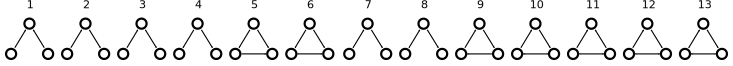
\includegraphics[scale=1]{figures/triads}
		\caption{All triads---connected directed graphs with three vertices---, numbered from 1 to 13.}
		\label{fig:triads}
	\end{figure*}
	
	Previous work has shown that graphs from the same domain tend to be characterized by similar triad concentration profiles \cite{Milo2002}. For example, Figure \ref{fig:triads}(a) presents triad concentration profiles for two software dependency graphs, whereas Figure \ref{fig:triads}(b) presents triad concentration profiles for graphs in distinct domains: a software dependency graph and a linguistic graph. An informal analysis reveals that the similarity between the profiles is greater in the first case. It should suffice to notice that, in the second case, the concentration of the first two triads is somewhat reversed (in the linguistic graph, the second triad is the most frequent).

	\begin{figure*}[htbp]
		\centering
			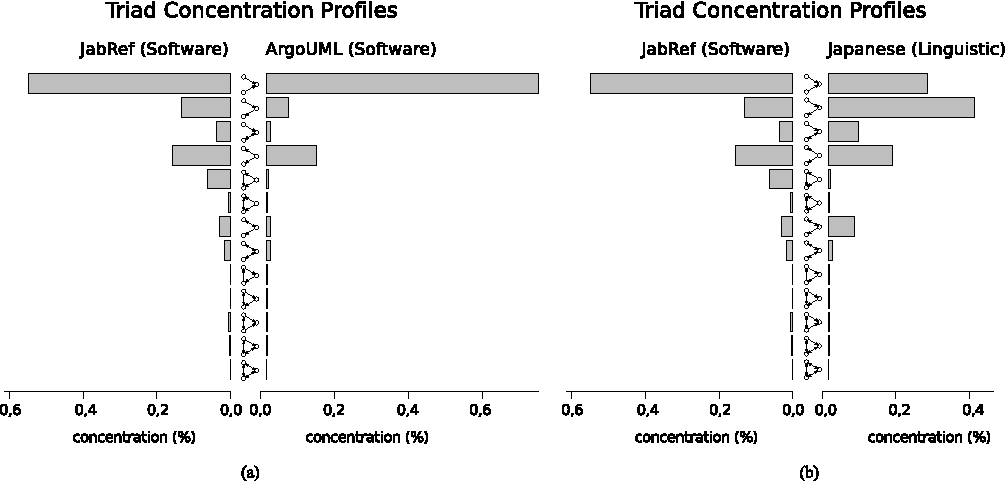
\includegraphics[scale=1]{figures/tcp}
		\caption{Comparison between triad concentration profiles for three distinct graphs (computed with the igraph tool \cite{igraph}). (a) Class dependency graphs for two softwares: JabRef, version 2.5b2 (left) and ArgoUML version 0.28 (right). (b) Graph for JabRef, version 2.5b2 (left), and graph of word succession in a sample of Japanese texts (right) \cite{Milo2004}.}
		\label{fig:tcp}
	\end{figure*}
	
	Many authors \cite{Milo2004,Ma2007,Lin2008} have explored triad concentration profiles as a means to find clusters of structurally similar graphs. The results suggest that such profiles can be effectively used to identify groups of graphs from the same domain (e.g., social, linguistic, biologic etc.).
			
\end{subsection}

\begin{subsection}{Graph Classifier}

We propose a classifier, based on triad concentration profiles, that, given a graph, determine if it is software-realistic (i.e., if it is likely to be a software dependency graph). The classifier is developed by a neural network on a data set containing both software and non-software graphs. We show that it is capable of classifying correctly most graphs.

% In order to determine whether triad concentration profiles are indeed effective in distinguishing software dependency graphs from other graphs, we use them as parameters of ... \TODO

\begin{subsubsection}{Data Set} \label{sec:data-set}
	
	In order to train our classifier, we have collected 131 graphs, including software dependency networks and graphs from other domains.
	
	We have collected 66 directed graphs that were made available by researchers working on domains such as biology, sociology, technology, and linguistics. The size of these graphs range from 32 to 18,163 vertices. The complete list of graphs can be found in Appendix A. % TODO
	
	Also, we have collected 65 open source software systems written in Java and listed at SourceForge.net\footnote{\url{http://sourceforge.net/about}} among the most popular as of 2008. From each software system one dependency graph was extracted, as follows.
	
	The archive for each software system contained one or more JAR files (Java Archive), containing object code for each class or interface. Some JAR files were generic libraries used by the systems; these files were removed from the extraction, as they are not really part of the software and are not considered by architecture recovery algorithms.
	
	Then, we used the tool Dependency Finder\footnote{\url{http://depfind.sf.net/}} in order to extract dependencies between classes (or interfaces) from the remaining JAR files. This particular tool was chosen because of the ease of use from the command-line, enabling its integration in scripting environments. We believe that any other tool with the same purpose would produce similar outputs.
	
	The graphs that were extracted contain vertices representing Java classes and interfaces. The edges represent any reference from one class/interface to another in the object code, including inheritance, aggregation, method call, object instantiation and attribute read/write.
	
	After the extraction process, we ended up with 65 software dependency graphs, with sizes ranging from 63 to 6,433 vertices. More information about these graphs can be found in Appendix A. % TODO
	
	For each of the 131 graphs, we extracted its triad concentration profile using the tool igraph \cite{igraph}. No other information about the network (such as number of vertices or number of edges) was used to build the classifier.

\end{subsubsection}

\begin{subsubsection}{Training and Evaluation}
	
	The data set with 131 graphs (65 software dependency graphs, 66 graphs from other domains) was used to a neural network classifier. To this end, each software dependency graph was labelled as software-realistic, and the other graphs were labelled as non software-realistic. 
	
	We chose, for the neural network, a multilayer perceptron with one hidden layer containing 7 nodes. First, we trained the neural network on the full data set with 131 graphs. Then, in order to obtain a reasonable estimation of the performance of the neural network, we used 10-fold stratified cross-validation.
	
	In 10-fold stratified cross-validation, the data set is split randomly in 10 folds (or parts), so that, in each fold, approximately half of the graphs are software-realistic (so as to reflect the proportions of each class in the full data set). Then, in each iteration, one fold is chosen as the test set, so that a neural network is trained on 9 folds and its performance is evaluated by having it try to predict the class of the graphs in the fold that is the test set. This way, each graph is used only once for testing purposes, so standard performance metrics such as precision and recall can be computed.
	
	\TODO We use the technique of random data splitting to measure the ability of the change burst metrics to predict defect- proneness. The data splitting technique is employed to get an independent assessment of how well the defect-proneness could be estimated from a population sample. 
	
	\TODO Precision and recall
	
	%  set and the remaining folds comprise the training set. That way, in each iteration, one neural network is trained (on the training set), and its performance is evaluated on the test set. 
	% 
	% In order to evaluate the performance of these classifiers, we used 10-fold stratified cross-validation. 
	
	% weka.wikispaces.com/Primer
	% A more elaborate method is cross-validation. Here, a number of folds n is specified. The dataset is randomly reordered and then split into n folds of equal size. In each iteration, one fold is used for testing and the other n-1 folds are used for training the classifier. The test results are collected and averaged over all folds. This gives the cross-validation estimate of the accuracy. The folds can be purely random or slightly modified to create the same class distributions in each fold as in the complete dataset. In the latter case the cross-validation is called stratified. Leave-one-out (loo) cross-validation signifies that n is equal to the number of examples. Out of necessity, loo cv has to be non-stratified, i.e. the class distributions in the test set are not related to those in the training data. Therefore loo cv tends to give less reliable results. However it is still quite useful in dealing with small datasets since it utilizes the greatest amount of training data from the dataset.
	
\end{subsubsection}

\begin{subsubsection}{Results}
	
	We evaluated the precision and recall of the graph classifier using the previously explained 10-fold cross-validation method. We obtained both a precision and a recall of 95.4\%, which is an excellent result.
	
	% The interpretation is that, given a graph that was classified as software-realistic, the probability of error (that is, the false positive rate) is about xxx\%. -- In fact we cannot know the false positive rate without knowing the true positive and true negative rate.
	
	We also trained a logistic regression model and neural networks with more nodes and more hidden layers, but none of these outperformed the simple neural network with one hidden layer containing 7 nodes.
	
	% Increasing the number of nodes or the number of layers did not yield better results. We also have trained a logistic regression model, that performed slightly worse than the neural network.
	
\end{subsubsection}

\end{subsection}
	
\end{section}

\begin{section}{BCR+ Evaluation}
	In the previous subsection, we have proposed a graph classifier that determine, with high precision and recall, whether a graph is software-realistic. In this section, we evaluate whether the BCR+ graph model is able to synthesize software-realistic graphs. The evaluation process is divided in three steps:
	
	\begin{enumerate}
		\item \emph{parameter selection}: by varying the values of the parameters of the model, we come to thousands of possible parameter configurations, so to explore the variety of graphs that can be synthesized;
		
		\item \emph{graph synthesizing}: for each parameter configuration, we synthesize three graphs, in order to mitigate the effect of randomness in the synthesis process;
		
		\item \emph{graph classification}: each graph is classified (using the previously built graph classifier) as software-realistic or non software-realistic.
	\end{enumerate}
	
\begin{subsection}{Parameter Selection}
	To synthesize a large variety of graphs, we have varied the value of each parameter from BCR+ so as to cover a wide range of possible values. Each assignment of values to parameters is called a configuration. We have chosen configurations for each possible combination of the selected parameter values.
	
	\TODO we also tried to keep the number of values for each parameter low, to avoid combinatorial explosion that would render the evaluation infeasible. 
	
	To recap, BCR+ has seven parameters: the number of vertices, $n$; the reference architecture, $G$; three complementary probabilities, $p_1$, $p_2$, and $p_3$; the mixing probability, $\mu$; and nonnegative values $\din$ and $\dout$. The probabilities are bounded parameters, with values ranging from 0.0 to 1.0. The remaining parameters are more complex.
	
	We have fixed the number of vertices, $n$, to 1,000, a value that has been used in related work \cite{Lancichinetti2009b}. To fix the number of vertices should not influence the results, since it affects only the size of the graph, not the pattern of connections between vertices.
	
	The parameter $G$ is the most complex, because it determines not only the number of modules, but also the interconnection between these modules. It should be noted that, with only three modules, there are 13 possible values for $G$ in which no module is isolated from the others.
	
	In order to avoid arbitrary graphs for $G$, we have instead used graphs that were extracted from software systems from the data set described in section \ref{sec:data-set}. For this task, we have extracted dependencies for all JAR files bundled with the system, including library files. Then, we have considered that each JAR is a module and that dependencies from entities in one JAR to entities in another JAR represent dependencies between modules. We believe that JAR files are good surrogates to modules, because distinct JAR files usually correspond to the work of distinct development teams.
	
	In the end, 5 graphs were chosen as $G$, with sizes from 2 to 32 modules. The graphs were extracted from the following software systems: GEF (2 modules), iBATIS (4 modules), MegaMek (8 modules), findbugs (16 modules), and zk (32 modules).
	
	For the parameters $p_1$, $p_2$, and $p_3$, we have chosen values in the set $\{0.0, 0.2, 0.4, 0.6, 0.8, 1.0\}$, such as $p_1 + p_2 + p_3 = 1.0$. Also, we determined that $p_1 + p_2 > 0$, because $p_1$ and $p_2$ correspond to rules that add vertices (otherwise, the graph would not grow in number of vertices).
	
	For the parameter $\mu$, we have selected values from the set $\{0.0, 0.2, 0.4, 0.6\}$. Because $\mu$ controls the proportion of external edges, that connect vertices from distinct modules, we avoided high values, that would lead to highly coupled graphs.
	
	For the parameters $\din$ and $\dout$, we have selected values from the set $\{0, 1, 2, 3, 4\}$. The values are somewhat arbitrary, but we avoided high values, because they would render graphs in which the distribution of edges per vertex is more homogeneous, unlike the distribution for software dependency graphs.
	
	For the selected parameter values, there are 9,500 configurations.
	%For unbounded parameters, we have chosen values based on the literature or grounded in the observation of software dependency graphs.

\end{subsection}

\begin{subsection}{Graph Synthesis and Evaluation}
	
	
	
\end{subsection}

	4,517 networks (15.8\% of 28,500) were classified as software-realistic, a result better than chance.
	
	\TODO for comparison, we have built random graphs. None was considered software-realistic.
	
	\TODO build a predictor of the software-realism based on BCR+ parameters?
	
\end{section}

%%%%%%%%%%%%%%%%%%%%%%%%%%%%%%%%%%%%%%%%%%%%%%%%%%%%%%%%%%%%%%%%%%%%%%%%%%%%%

\begin{section}{Evaluation of Architecture Recovery Algorithms}
	\TODO Clustering

	\TODO Brief description about Bunch, ACDC, SL75/SL90, CL75, CL90
	
	\TODO Traditional experimental setup for evaluation of architecture recovery algorithms: given a dependency graph and a reference architecture, run the algorithm on the graph and compare the recovered architecture with the reference architecture.
	
	\TODO MoJo metric.

\begin{subsection}{Experimental Setup}
	\TODO Section 6.3 from dissertation
\end{subsection}

\begin{subsection}{Comparison of Architecture Recovery Algorithms}
	% Section 6.4 from dissertation
	
	The first experiment was aimed at comparing the performance of the algorithms when applied software-realistic graphs, measured by the similarity between the clusters found by the algorithms and the modules of the reference architecture.
	
	We have selected for this experiment only the graphs that were classified as software-realistic, totalizing about 6,000 graphs. Then, each algorithm was applied to each one of the synthetic graphs, resulting in a set of clusters together with a mapping from the set of vertices to the set of clusters. The performance of the clusterings were measured with the metric MoJoSim.
	
	The Figure \ref{fig:exp-algorithms} shows a boxplot of the MoJoSim values that were measured for each algorithm. The dashed lines indicate the maximum and minimum value from the data. Comparing the median performance of the algorithms, it is clear that ACDC presents the best performance, followed by Bunch, and then by the hierachical algorithms. These differences were verified to be significative by applying a paired Wilcoxon test ($\alpha = 0.05$), with Bonferroni correction to account for multiple hypothesis testing. Among the hierarchical algorithms, there was no evidence that their performances differ.
	
	\begin{figure}[htbp]
		\centering
			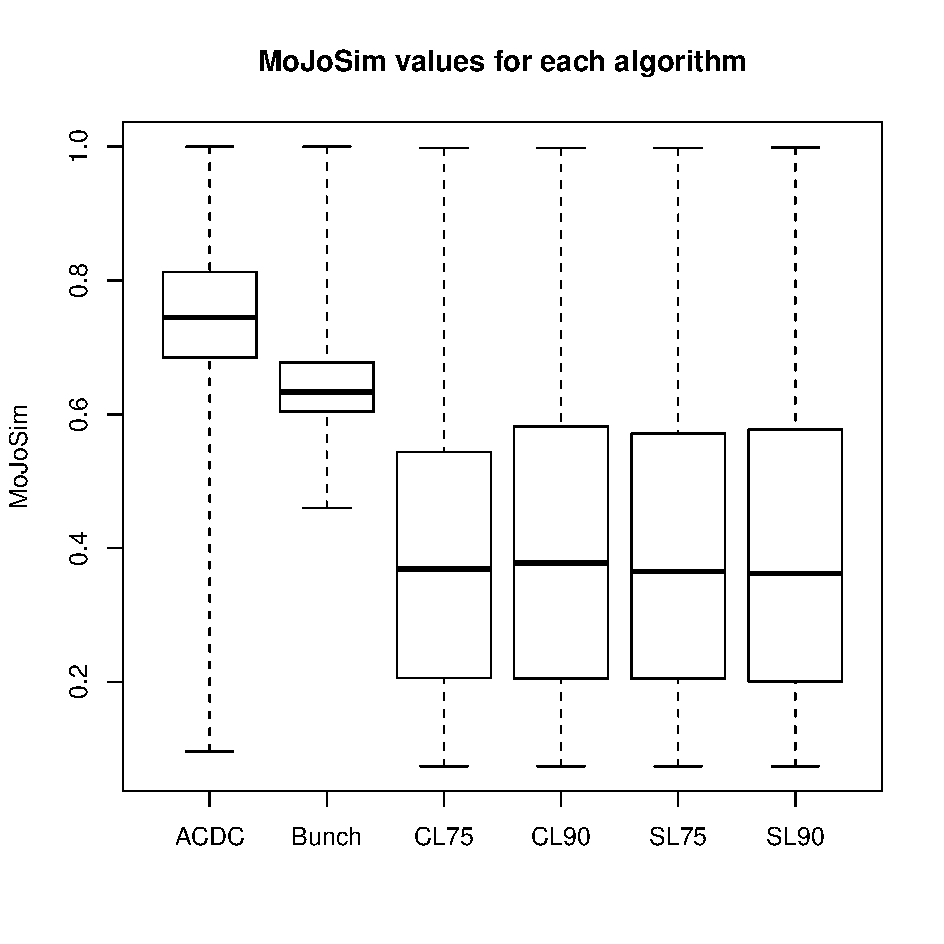
\includegraphics[width=0.5\textwidth]{figures/exp-algorithms}
		\caption{Statistical summary of MoJoSim values for each architecture recovery algorithm.}
		\label{fig:exp-algorithms}
	\end{figure}
	
	Another noteworthy aspect of the data is the dispersion of values. The algorithm Bunch presents the smaller dispersion, with more that half of the values between 0.60 and 0.80 (minimum value = 0.45). In the case of ACDC, half of the values are between 0.65 a 0.85, but the minimum value is 0.01. This observation suggests that, although Bunch presents overall inferior performance when compared with ACDC, it can be a resonable choice for yielding more predictable results.
	
	\TODO move to a discussion section.
	The results disagree with conclusions from Wu, Hassah, and Holt \cite{Wu2005}. They have concluded that the SL algorithms outperform ACDC, which outperforms Bunch, which outperforms the CL algorithms. The disagreement probably can be explained by the criteria they used to build the reference architecture for each software system. They use the folder structure from the source of the software system to determine the modules in the architecture reference. In our work, the reference architecture is defined a priori, and the graphs are synthesized ro reduce the dependencies between modules.
	
	We should note that this experiment suffers from sampling bias. Although all analyzeds graphs are software-realistic, we can not guarantee that it is representative of all software systems. We see this analysis as complementary to similar experiments, that suffer from other types of bias \cite{Wu2005,Bittencourt2009,Andritsos2005}.
	
\end{subsection}	

\begin{subsection}{Algorithm Parameters Analysis}
	% Section 6.5 from dissertation
	
	In the next experiment, we tried to understand how the algorithms behave on a variety of situations---graphs with different number of modules, different proportions of external edges etc. We were able to control a number of graph properties by changing parameter values for the BCR+ model.
	
	In this experiment, all graphs---both software-realistic and non software-realistic---were considered, in order to avoid the software-realism variable to bias the results.
	
	We have analyzed the influence of the number of modules and of the proportion of external edges on the performance of the algorithms. We have chosen these two properties because they map naturally to BCR+ parameters: number of modules is controlled by the input module graph, $G$, and proportion of external edges is controlled by the parameter $\mu$.

	\TODO explain that the sample is paired, that is, there are two graphs that differ only by $\mu$ (the other parameters are identical).
	
	\TODO this experiment is not possible with traditional approaches, since it depends on having control on the graphs properties.
	
	As expected, all algorithms performed better when the proportion of external edges was smaller. \TODO is it true? Check experimental package
	
	A surprising result was found when analyzing the influence of the number of modules on the performance of the algorithms (see Figure \ref{fig:exp-number-modules}). While the performance of ACDC and Bunch are not influenced by the number of modules, the performance of the hierachical algorithms is worse when applied to graphs with more modules. In fact, the performance of such algorithms are comparable to the performance of ACDC and Bunch when there are only two modules, but it gets  progressively worse as the number of modules grows.
	
	\begin{figure}[htbp]
		\centering
			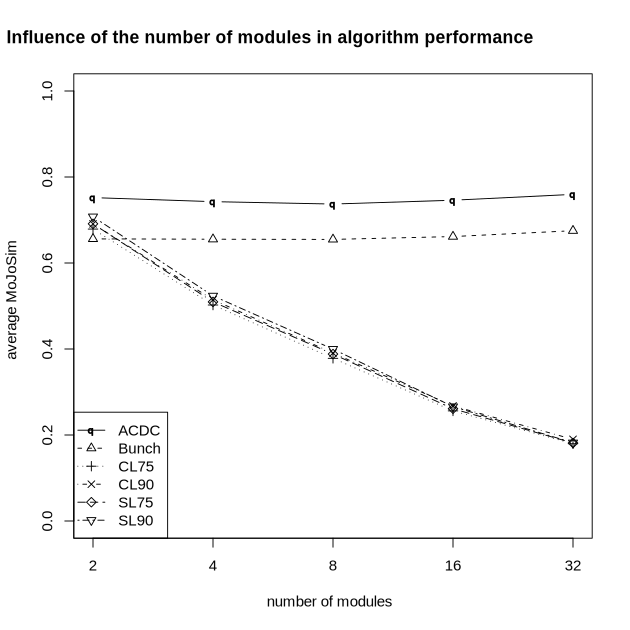
\includegraphics[scale=0.5]{figures/exp-number-modules}
		\caption{Influence of the number of modules in the reference architecture on the performance of each architecture recovery algorithm.}
		\label{fig:exp-number-modules}
	\end{figure}
	
	A possible explanation for this phenomenom can be found in the distribution of module sizes found by hierarchical algorithms. It is common that they found large modules, sometimes covering more than half of the vertices \cite{Wu2005}. If the reference architecture contains many smaller modules, large modules found by an algorithm are severely penalyzed by the MoJoSim metric (the large modules need to be split in smaller modules, which is accounted in MoJoSim as a sequence of vertex movimentations).
	
\end{subsection}

\begin{subsection}{Impact of Bidirectional Dependencies}
	% Section 6.6 from dissertation
	
	The third experiment was aimed at measuring the influence of the type of dependency (unidirectional of bidirectional) on the performance of each architecture recovery algorithm. The independent variable is the parameter $G$ from BCR+, that is, the definition of the modules and allowed dependencies between modules.
	
	We have analyzed two configurations for $G$:
	
	\begin{itemize}
		\item \emph{bidirectional}: $G$ contains two modules, $M_1$ and $M_2$; there is a bidirectional edge between $M_1$ and $M_2$ (that is, vertices in $M_1$ may depend on vertices of $M_2$ and the other way around);
		
		\item \emph{unidirectional}: $G$ contains two modules, $M_1$ and $M_2$; there is an unidirectional edge from $M_1$ to $M_2$ (that is, vertices in $M_1$ may depend on vertices of $M_2$, but the opposite is not true).
	\end{itemize}
	
	As far as we know, BCR+ is the only graph model that can be used to conduct this type of experiment. Other graph models do not offer control over specific dependencies.
	
	For the remaining parameters of BCR+, when considered the values described in Section XXX. For each configuration of parameters, three graphs were synthesized, totalizing 11,400 graphs. Then, each architecure recovery algorithm was applied to each graph. Finally, the performance was computed, using the metric MoJoSim.
	
	The results are shown in a boxplot in Figure \ref{fig:exp-dependencies}. It can be observed that all algorithms performed slightly better on the graph with the unidirectional edge. All differences---except that of CL75---are significative at 5\% level, as assessed with the paired Wilcoxon test.
	
	\begin{figure*}[htbp]
		\centering
			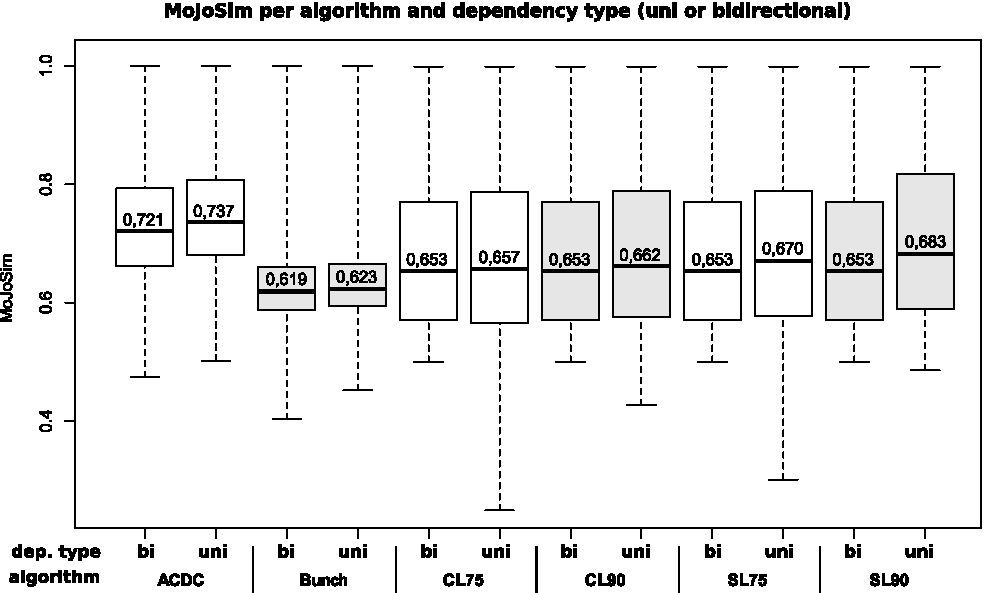
\includegraphics[scale=1]{figures/exp-dependencies}
		\caption{Influence of the type of dependency between modules (unidirectional ou bidirectional) on the performance of each architecture recovery algorithm.}
		\label{fig:exp-dependencies}
	\end{figure*}
	
	The difference of performance for each algorithm is shown in Table \ref{tab:exp-dependencies}, as a 95\% confidence interval. ACDC and SL75 are more influenced by the choice of dependency type than the other algorithms. Overall, the difference between MoJoSim values does not exceed 0.03 (except in the case of SL90), which is a small value.
	
	\begin{table*}[width=\textwidth]
	  \begin{center}
	  \begin{tabular}{cccccc}
	    \hline
	    \textbf{ACDC} & \textbf{Bunch} & \textbf{CL75} & \textbf{CL90} & \textbf{SL75} & \textbf{SL90} \\
	    \hline
	    \hline
	    \footnotesize{[0,016; 0,023]} & \footnotesize{[0,004; 0,008]} & \footnotesize{[-0,004; 0,006]} & \footnotesize{[0,006; 0,015]} & \footnotesize{[0,007; 0,017]} & \footnotesize{[0,021; 0,031]} \\
	    \hline
	  \end{tabular}
	  \end{center}
	  \caption{Intervalo de confiança de 95\% para a diferença de desempenho de cada algoritmo, medido em MoJoSim, entre a configuração \emph{simples} e a configuração \emph{dupla} do parâmetro G.}
	  \label{tab:exp-dependencies}
	\end{table*}
	
	We conclude that, in general, the presence of modules with mutual, bidirectional dependencies, influences negatively the performance of the algorithms that were analyzed. The observed difference was small in our study with two modules, but we suspect that this difference can be greater on graphs with more modules and more bidirectional dependencies.
	
\end{subsection}

\begin{subsection}{Discussion}
  % TODO: move to a new section
	We have described three experiments based on the application of architecture recovery algorithms to synthetic graphs created by the model BCR+. The experiments present evidence that this approach is practicable and can be used to find insights about the algorithms that cannot be found with more traditional approaches.
	
	\TODO more
	
\end{subsection}

\end{section}

%%%%%%%%%%%%%%%%%%%%%%%%%%%%%%%%%%%%%%%%%%%%%%%%%%%%%%%%%%%%%%%%%%%%%%%%%%%%%

\begin{section}{TODO: Other Possible Sections}
	Discussion
	
	Limitations: selection bias for training the classifier. selection bias for synthesized graphs.
	
	Related work: evaluation of Bunch using random graphs. Lancichinetti's evaluation of clustering algorithms using his network model. Evaluation of architecture recovery algorithms by comparing recovered modules with packages that are explicit in source code. (TODO: maybe promote to 2nd section)
	
	Conclusion
	
	Acknowledgments
	
	References	
\end{section}

%%%%%%%%%%%%%%%%%%%%%%%%%%%%%%%%%%%%%%%%%%%%%%%%%%%%%%%%%%%%%%%%%%%%%%%%%%%%%
%%%%%%%%%%%%%%%%%%%%%%%%%%%%%%%%%%%%%%%%%%%%%%%%%%%%%%%%%%%%%%%%%%%%%%%%%%%%%

\bibliographystyle{plain}
\bibliography{ase2012-reference-arch}

\end{document}
